\documentclass[11pt,a4paper]{article}
\usepackage{a4wide,url,graphicx}
\usepackage[utf8]{inputenc}
\usepackage[main=german,russian]{babel}

\parindent0pt
\parskip3pt
\newcommand{\ergaenzen}{\textbf{Ergänzen.}\ }

\title{TRIZ-Anwendung beim Architekturentwurf eines\\ Steuerungssystems auf
  der Grundlage von\\ Daten in der Energietechnik}

\author{A.P. Tjukow, Staatliche Technische Universität Wolgograd, Russland}

\date{TRIZ-Summit 2020}

\begin{document}
\maketitle

\begin{quote}
  Der Aufsatz wurde auf dem TRIZ-Summit 2020 präsentiert. Das Original ist
  unter
  \url{https://r1.nubex.ru/s828-c8b/f3137_9d/Tyukov-TDS-2020.pdf}
  zu finden.

  Übersetzung ins Deutsche von Hans-Gert Gräbe, Leipzig.
\end{quote}

\begin{abstract}
  In diesem Aufsatz werden die Erfahrungen mit der Visualisierung der
  Architektur eines Steuerungssystems auf der Grundlage von Energiedaten
  (SUND) und der Strategie seiner weiteren Entwicklung unter Anwendung von
  TRIZ-Instrumenten beschrieben: Funktionsanalyse, Ursache-Wirkungs-Analyse
  CECA, Suche nach Unzulänglichkeiten und Methoden zu deren Beseitigung.  SUND
  dient der Verwaltung von Informationsflüssen in der Energiewirtschaft:
  Heizungsmanagement auf der Basis von Wettervorhersagen, Lademanagement von
  Elektrofahrzeugen, Management von Energieflüssen in verteilten
  Energiesystemen, technisch-ökonomische Machbarkeitsstudien. Bei der Analyse
  und Beschreibung der neuen Systemarchitektur wird mit Notationen aus den
  Bereichen UML, BPMN, Archimate, Datenflussdiagramme (DFD) in der
  Systemmodellierungsumgebung \emph{Visual Paradigm} unter Verwendung der
  TOGAF-Methodologie gearbeitet.  Der Autor stellt eine Hypothese über
  verallgemeinerte Mängel und Methoden zu deren Beseitigung bei der Bildung
  von datenbasierten Steuerungssystemarchitekturen auf.

  \emph{Schlüsselworte:} Informationssysteme, Architekturen, TRIZ,
  datengetriebene Steuerung, System Engineering.
\end{abstract}

\section*{1. Einführung}
Datenbasierte Steuerungssysteme gehöern zur Kategoie der komplexen Systeme,
weil eine Person nicht in der Lage ist, deren Beschreibung unter Verwendung
von existierenden Werkzeugen zu überschauen [1].

In diesem Artikel betrachten wir die Architektur eines Steuerungssystems auf
der Grundlage von Energiedaten, die über 10 Jahre von mehr als 50 Entwicklern
entwickelt wurde: die Nutzer der Produkte, die Entwickler, die
Finanzierungsprogramme und die Technologie haben sich geändert, aber die
Architektur war bisher nicht beschrieben und es gab auch keine Standards.  Die
Unternehmensentwicklung hat sich beschleunigt, woraus zusätzliche
Anforderungen an die Architektur des datenbasierten Steuerungssystems
erwachen.

Ziel des Artikels ist es, über Erfahrungen bei der Beschreibung und
Entwicklung dieses datenbasierten Steuerungssystems auf der Basis des
Einsatzes von TRIZ-Instrumenten zu berichten. Er besteht aus folgenden
Abschnitten:
\begin{enumerate}
\item[1)] Analyse der Aufgabe des Entwurfs der Architektur des datenbasierten
  Steuerungssystems.
\item[2)] Lösungsbeschreibung: Dieser Abschnitt beschreibt die Hauptidee der
  vorgeschlagenen Lösung.
\item[3)] Diskussion und Schlussfolgerungen: Dieser Abschnitt enthält die
  vorgeschlagene Liste der Nachteile und Techniken zu ihrer Beseitigung.
\item[4)] Ergebnisse der Einführung.
\end{enumerate}
Die Autoren gehen davon aus, dass der Einsatz der TRIZ es ermöglicht, die
Effizienz der Entwicklung des datenbasierten Steuerungssystem zu erhöhen. Sie
stellen eine Hypothese über das Vorhandensein von Heuristiken bei der
Entwicklung von Informationssystemen auf, ähnlich den 30 Mängeln, die von
V. Lenyashin thematisiert wurden, und den 40 Prinzipien zur Beseitigung von
Widersprüchen in der „eisernen“ TRIZ [2], [3], [4].

\section*{2. Analyse der Aufgabe}

Vor der Einführung der beschriebenen Methoden verwendeten die Mitarbeiter des
Unternehmens verschiedenartige, nicht zusammenspielende Werkzeuge zum
Entwerfen, Implementieren und Dokumentieren von datenbasierten
Steuerungssystemen, die technologischen Anforderungen waren nicht beschrieben,
was zu folgenden Nachteilen führt:
\begin{itemize}
\item[1)] Die Entwickler haben eine enge Sicht auf das Gesamtsystem, aber
  tiefes Wissen über den eigenen Bereich, was zur ständigen Auseinandersetzung
  über die Systemarchitektur, über verwendete Komponenten, zu Redundanz von
  Funktionalität und zu häufigem Uminterpretieren und Umschreiben des Systems
  führt. 
\item[2)] Das Fehlen eines einheitlichen Glossars wirkte sich negativ auf den
  Prozess des Entwurfs der Lösungsarchitektur aus, es gab Fragen bei der
  Definition von Begriffen wie Produkt, Service, Vereinbarung,
  Service-Level-Vereinbarung usw.
\item[3)] Es wird eine größere Zahl verschiedener Visualisierungsprogramme der
  Architektur verwendet: Draw.io, Visio, Flying Logic. Damit ist es nicht
  möglich, Diagramme anderer Projekte wiederzuverwenden und Projekte zwischen
  Teilnehmern auszutauschen.
\item[4)] Das Fehlen des beschriebenen technischen Systems erlaubt es nicht,
  „due diligence“ in Großprojekten durchzusetzen.
\end{itemize}
Vor der Enticklung der Anwendungsarchitektur wurden folgende Anforderungen
identifiziert:
\begin{itemize}
\item[(i)] Das Programm sollte das System modellieren, nicht Diagramme
  zeichnen,
\item[(ii)] Arbeit mit Beschreibungsebenen des technischen Systems,
\item[(iii)] Wiederverwendung von Objektbeschreibungen,
\item[iv)] alle entwickelten Diagramme können in einer Datei gespeichert
  werden,
\item[v)] Unterstützung von Repositories und gemeinsames Speichern und
  Bearbeiten der Architektur soll online möglich sein.
\end{itemize}
Die Entwickler haben \emph{Visual Paradigm} gewählt als einziges Programm, das
diese Anforderungen erfüllt.

Als Prototyp des Entwurfsprozesses für die Architektur wurde der Prozess der
Ausbildung zum TRIZ-Master von Yuri Danilovsky in funktioneller Analyse
verwendet, der aus den folgenden Etappen besteht:
\begin{itemize}
\item[1)] Durchführen einer Funktionsanalyse in der Notation von Miles.
\item[2)] Bestimmung einer Liste von Defiziten.
\item[3)] Durchführung einer Ursache-Wirkungs-Analyse der Primärursachen,
  Entwurf einer Liste fehlender Komponenten.
\end{itemize}
\begin{center}
  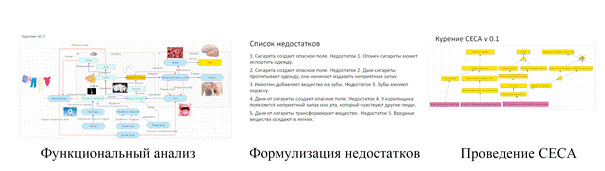
\includegraphics[width=.95\textwidth]{image002.jpg}\\
  \textbf{Abbildung 4}. Durchführen einer Funktionsanalyse an einem
  Trainingsbeispiel für Zigaretten, verfasst von Anton Tyukov.
\end{center}
In der beschriebenen Lösung werden anstelle von Funktionsanalysediagrammen
Datenflussdiagramme (DFD) als Werkzeug zur Informationsflussanalyse verwendet.
In der Arbeit wird der Begriff des Defizits anstelle des üblichen
TRIZ-Begriffs des Widerspruchs verdendet, weil Widersprüche für unvorbereitete
Menschen schwer wshrzunehmen sind.

\section*{3. Beschreibung der Lösung}

Die vorgeschlagene Methodik ermöglicht eine Strukturierung des Prozesses der
Entwicklung einer datenbasierten Steuerungssystems, Reduzierung der
Komponentenduplikation, Reduzierung der Transaktionskosten bei der
Kommunikation disziplinübergreifender geografisch verteilter Befehle und
basiert auf:
\begin{itemize}
\item[1)] Verwendung des Beschreibungsstandards TOGAF für
  Organisationsarchitekturen, um Aspekte der Aufmerksamkeit beim Entwurf der
  Unternehmensarchitektur zu definieren.
\item[2)] Visualisierung einzelner Aspekte des Systems auf der Grundlage der
  Anwendung allgemein anerkannter Standards für die visuelle Modellierung von
  datenbasierten Steuerungssystemen:
  \begin{itemize}
  \item[(a)] Datenflussdiagramme (DFD als Analog der Funktionsanalyse für
    Informationssysteme);
  \item[(b)] BPMN für die Prozessbeschreibung, Archimate für die
    Visualisierung von Organisationsarchitekturen.
  \item[(c)] Prinzipien der Funktionsanalyse von technischen Systemen in der
    Notation von Miles, die auf Informationssystem-Architekturen und die
    DFD-Notation übertragen werden.
  \item[(d)] Prozess der Defizitsuche auf der Grundlage der TRIZ-Notationen
    und der Methoden zu ihrer Beseitigung.
\end{itemize}
\end{itemize}
Die Umsetzung der Methodik zur Entwicklung von datenbasierten
Steuerungssystemen besteht aus den folgenden Schritten:
\begin{itemize}
\item[1)] Erstellung einer Liste von Software, die im firmeninternen
  Software-Ökosystem datenbasierter Steuerungssysteme verwendet wird, sowie
  einer Liste von Mitarbeitern, die für die einzelnen Softwaren verantwortlich
  sind.
\item[2)] Erstellen eines Zeitplans für Treffen mit jedem der Entwickler zur
  Diskussion der Elemente der Systemarchitektur. Um sich ein vollständiges
  Bild zu machen, sind mehrere Iterationen der Durcharbeitung der von den
  Mitarbeitern verwendeten Funktionalität erforderlich.
\item[3)] Erstellen synthetisierender Diagramme, mit denen sich die erstellte
  Architekturbeschreibungen zusammenfassen und gruppieren lassen.
\item[4)] Erstellung eines vollständig vereinheitlichten, vollständig
  synthetischen Diagramms, welches das Konzept eines datenbasierten
  Steuerungssystems beschreibt, das 
  \begin{itemize}
  \item[(i)] einen Überblick über das Informationssystem zur datenbasierten
    Steuerung in einem für den Nichttechnologen verständlichen Format gibt
    sowie
  \item[(ii)] das Zugriffsrouting für Diagramme
  \end{itemize}
  erlaubt.
\item[5)] Durchführung einer datenbasierten Analyse des gesamten Ökosystems
  der datenbasierten Steuerungsysteme zur Identifizierung von Defiziten sowie
  Durchführung einer Ursachen-Wirkungs-Analyse für den Übergang in den Zustand
  „Wie es sein sollte“.
\item[6)] Zusammenstellen einer Gruppe von Diagrammen „Wie es sein sollte“ des
  Idealzustandes des Systems, basierend auf einer Analyse des Ist-Zustandes.
\item[7)] Erstellung eines Online-Repositoriums für die gemeinsame Arbeit mit
  Diagrammen.
\item[8)] Veröffentlichung der Ergebnisse der Diagrammerstellung in Form einer
  einzigen html-Datei im Benutzer-Ökosystem, um Informationen im
  Firmen-Ökosystem anzuzeigen.
\item[9)] Schulung der Mitarbeiter für die Arbeit mit dem System.
\end{itemize}
Nach einer Iteration auf der Basis der Analyse technischer Systeme ist der
Übergang zu einer umfassenderen Sicht der Architektur der Organisation zum
Zweck der Synchronisierung der entwickelten Beschreibung der Programmteile der
Architekturen mit dem Kundengeschäft und der technische Implementierung
möglich.

\section*{4. Ergebnisse der Implementierung}
Während des dreimonatigen Projekts wurden über 80 Diagramme erstellt, um das
Wesen der verschiedenen Ebenen des Systems im Zustand „wie es ist“, „wie es
sein sollte“ zu offenbaren.  Darunter waren Diagramme, die den Prozess der
Umwandlung und Erhaltung der Systemarchitektur beschreiben. Die
Organisations-Ebenen wurden auf der Grundlage der Empfehlungen der
TOGAF-Methodologie modelliert: Geschäftsebene, Daten- und Anwendungsschicht,
Technologie-Ebene.

Innerhalb der Unternehmensebene wurden beschrieben: 
\begin{itemize}
\item[1)] Geschäftsprozesse des Kunden, die von dem in Entwicklung
  befindlichen datenbasierten Steuerungssystem profitieren,
\item[2)] Verkaufs- und Kundendienstprozess,
\item[3)] Beschreibung des Geschäftsprozesses der Entwicklung neuer
  Komponenten des Informationssystems. 
\end{itemize}
In den meisten Fällen wird die BPMN-Notation verwendet.

\begin{center}
  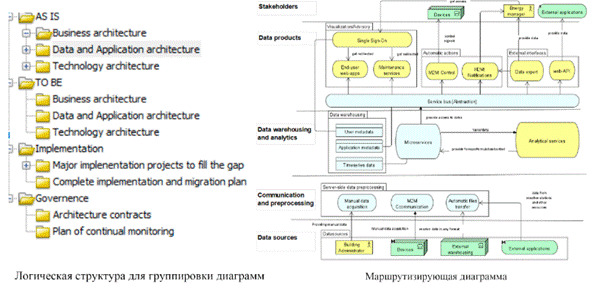
\includegraphics[width=.95\textwidth]{image004.jpg}\\
  \textbf{Abbildung 1}. Struktur und Routing der logischen Diagrammgruppierung
  Grafik (Ebene 1)
\end{center}
Diese Architektur ist logisch in die folgenden Funktionsblöcke unterteilt:
Datenquellen, Datenvorverarbeitung mit Integration, Datenspeicherung und
Analytik, datenbasierte Dienste. Dieses Diagramm wird nur zur Analyse der
Systemheit von Komponenten und das Routing von anderen Diagrammen verwendet,
die unter Beteiligung von Entwicklern erstellt wurden.

\begin{center}
  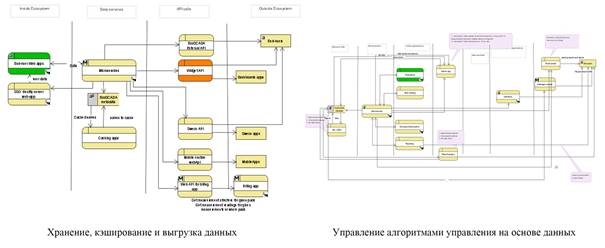
\includegraphics[width=.95\textwidth]{image006.jpg}\\
  \textbf{Abbildung 2}. Logische Darstellung der Datenarchitektur im System
  (Ebene 2)
\end{center}
\begin{center}
  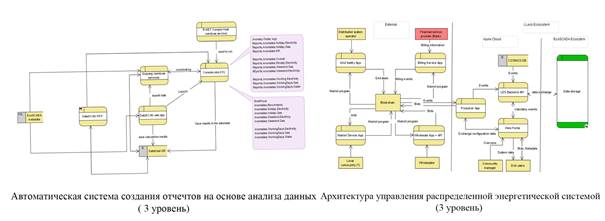
\includegraphics[width=.95\textwidth]{image008.jpg}\\
  \textbf{Abbildung 3}. Visuelle Beschreibung einiger ausgewählter
  Anwendungen (Ebene 3)
\end{center}
\begin{center}
  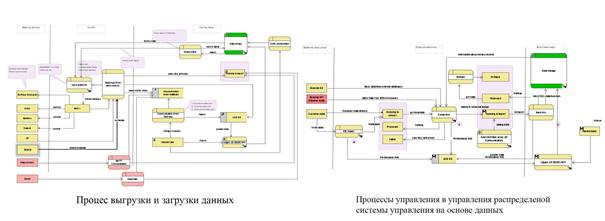
\includegraphics[width=.95\textwidth]{image010.jpg}\\
  \textbf{Abbildung 4}. Der Prozess des Hochladens, Herunterladens und
  Verwaltens verteilter Ausrüstungen.
\end{center}
\begin{center}
  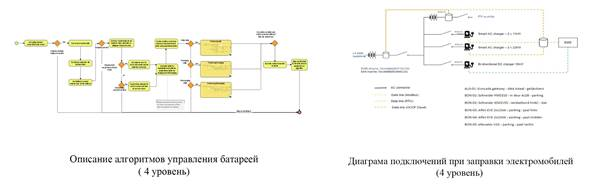
\includegraphics[width=.95\textwidth]{image012.jpg}\\
  \textbf{Abbildung 5}. Beispiele für die Beschreibung von
  Steuerungsalgorithmen und Anschlussplanungen
\end{center}

\section*{5. Diskussion und Schlussfolgerungen}

Im Rahmen der Untersuchungen wurde ein Systemglossar entwickelt, das es
ermöglicht, zu einer einheitlichen Sprache für die Beschreibung des Systems zu
kommen, sowie die Architektur entwickelt und visualisiert.  Das Vorhandensein
von Diagrammen hat den Aufwand bei der Erläuterung komplexer Aufgaben, bei der
Arbeitsverteilung unter den Entwicklern sowie bei der Formierung der
Strukturen in den Unternehmensabteilungen verringert.  Im Rahmen der Analyse
wurde eine Hypothese über die Liste von Defiziten in Architekturen
datenbasierter Steuerungssystem aufgestellt.  Zur Fehlerklassifizierung wurden
7 Kategorien aus dem System Engineering [2] verwendet: 
\begin{quote}
  i) Stakeholder, ii) Möglichkeiten, iii) Systemdefinition, iv)
  Systemimplementierung, v) Team, vi) Arbeit, vii) Technologie.
\end{quote}
Informationen mit einer Beschreibung der vorgeschlagenen Defizite und der Wege
zu deren Behebung sind in der folgenden Tabelle 1 zusammengestellt.

\begin{quote}
  \textbf{Tabelle 1:} Vorgeschlagene allgemeine Unzulänglichkeiten und
  Methoden zur Beseitigung von Defiziten in der IT
\end{quote}

\begin{center}\small
  \begin{tabular}{|p{.3\textwidth}|p{.3\textwidth}|p{.3\textwidth}|}\hline 
    Name des Fehlers & Ursache des Auftretens & Technik der
    Beseitigung\\\hline

    Geringe Operativität der Datenübertragung (Systemimplementierung) &
    
    Entsteht bei zu großer Anzahl von Vermittler-Komponenten,
    niedriger Durchsatzkapazität des Informationskanals,
    Besonderheiten technologischer Merkmale. &
    
    Die Anzahl der Vermittler-Komponenten verringern, Funktionen ins
    Obersystem auslagern, Caching verwenden.\\\hline
    
    Einsatz von Vermittler-Komponenten zur Datenverarbeitung
    (Systemimplementierung) & 
    
    Passiert, wenn die Entwickler ihre Arbeit nicht synchronisieren.&

    Aktivitäten der Entwickler koordinieren (gemeinsame
    Systemarchitektur).\\\hline 
  \end{tabular}
\end{center}
\begin{center}\small
  \begin{tabular}{|p{.3\textwidth}|p{.3\textwidth}|p{.3\textwidth}|}\hline 

    Komponenten doppelt (Systemimplementierung) &

    Entsteht, wenn es im Ökosystem mehrere Komponenten gibt, die dasselbe
    tun.&

    In Abstimmung mit den Entwicklern wird die Unterstützung einer der
    Komponenten beendet.\\\hline

    Geringe Abstimmung der Technologien (Technologie) &
    
    Passiert, wenn die gleiche Funktionalität in verschiedenen Komponenten
    implementiert wurde. &

    Erstellen eines unternehmensweit gültigen Architektur-Dokuments.\\\hline

    Funktionen wiederholen sich in verschiedenen Anwendungen
    (Systemdefinition) &
    
    Mehrere Anwendungen wiederholen komplett dieselbe Funktion. &

    Umverteilung der Funktionen zwischen den Komponenten, Entwurf des Systems
    nach funktionalen Gruppen.\\\hline

    Geringe Standardisierung auf der Technologie-Ebene (Technologie) &
    
    Anwendungen gleichen Typs sind in verschiedenen Sprachen entwickelt.  Es
    entstehen Probleme mit Vermittlung, Code-Weitergabe usw. &

    Erstellen einer unternehmensweit gültigen Architektur-Definition.\\\hline

    Fehlende Abstimmung der Funktionen auf Ökosystemebene (Systemdefinition) &

    Mehrere Anwendungen enthalten teilweise ähnliche Funktionen.  Für die volle
    Funktionalität muss der Nutzer mehrere Anwendungen aufrufen. &

    Umverteilung von Funktionen zwischen Komponenten in Übereinstimmung mit
    den Funktionsgruppen.\\\hline

    Unzureichende Durchsichtigkeit bei Entscheidungsfindung (Stakeholder) &

    Die Anwendung zeigt eine wichtige Informationen, aber es ist dem
    Benutzer nicht klar, was damit gemeint ist. &

    Übergang von der Entscheidungs-Unterstützung zum Entscheidungssystem, dem
    System ein Modul mit Hilfestellungen hinzufügen.\\\hline

    Überschüssiger Aufwand bei der Informationsbeschaffung (Stakeholder) &

    Für die rechtzeitige Informationsbeschaffung ist ein zu hoher Aufwand
    erforderlich. &

    Die Informationsbereitstellung muss über die für den Nutzer zugänglichsten
    Kanäle erfolgen: Smartphone, Email.\\\hline

    Geringe Motivation des Nutzers zur Nutzung der Anwendung (Stakeholder) &

    Tritt auf, wenn der Benutzer die eigentlichen Ziele des System nicht
    versteht. &

    Entwicklung eines Anreizsystems zur Verfolgung von Änderungen am.
    Rückkopplung in der Hilfe-Kommunikation einbauen, Bereitstellung von
    Statistiken und Gaminfication.\\\hline

    Vorbereitung der Daten vor de Analyse dauert zu lange (Team) &
    
    Die Datenaufbereitung erfordert zu viel Zeit. &

    Datenformate standardisieren Daten, automatisches System der
    Vorverarbeitung der Daten vor der Analyse einsetzen.\\\hline

    Fehlende Durchsichtigkeit der Kontrolle der technischen Prozesse (Team) &
    
    Es ist nicht klar, welche Komponenten des Systems aktuell arbeiten. &

    Erstellen eines Bündels Client-Server-Daten-Qualität für die ständige
    Überwachung der tatsächlichen Leistung entsprechend der Vereinbarungen mit
    dem Anwender.\\\hline
  \end{tabular}
\end{center}
\begin{center}\small
  \begin{tabular}{|p{.3\textwidth}|p{.3\textwidth}|p{.3\textwidth}|}\hline 

    Zu hohe Kopplung zwischen den Anwendungen (Team) &

    Anwendungen rufen sich während der Ausführung ohne hinreichenden Grund
    gegenseitig auf. Führt zur Verringerung der Systemstabilität. &

    Refactoring ausführen, Kopplung zwischen den Anwendungen
    verringern.\\\hline

    Zu geringe Informiertheit der Leitung über den aktuellen Stand der
    Architekturentwicklung (Stakeholder) &

    Ergebnis zu schneller Veränderungen, zu schlechter Qualität der
    Systembeschreibung, fehlendes System von Entwurf und Planung. &

    Standard der Systemkomponenten-Beschreibungen setzen.\\\hline

    Zu geringe Qualität der Komponenten (Systemimplementierung) &

    Während der Systemimplementierung entsteht die Frage nach alternativen
    Lösungen. &

    Implementierung eines Instruments zur Einschätzung der Qualität der
    Komponenten. \\\hline

    Zu geringe Geschwindigkeit der Änderungsanforderungen (kein Gebiet
    angegeben) &
    
    Verursacht durch zu geringe Geschwindigkeit der Entscheidungsfindung
    bzgl. Änderungsanforderungen durch das Management, führt zum Dublieren von
    Komponenten. & 
    
    Die Informiertheit der beteiligten Menschen erhöhen, Qualitätsstandards
    aufrechterhalten, schnell auf Änderungen reagieren.\\\hline
  \end{tabular}
\end{center}

Die vorgeschlagene Klassifizierung ist nicht umfassend, erlaubt es aber, die
psychologische Trägheit des Informationssystem-Architekten zu verringern. Die
vorliegenden Empfehlungen können angepasst und erweitert werden.

\section*{6. Schlussfolgerung}
In diesem Artikel schlugen die Autoren einen Weg zur Analyse und Verbesserung
der Arbeit von datenbasierten Steuerungssystemen unter Anwendung der
TRIZ-Methodik vor, formulierten Defizite im Prozess des Entwurfs und der
Weiterentwicklung der Systemarchitektur solcher Steuerungssysteme und schlugen
Wege vor, diese Defizite zu beseitigen. Die Autoren gehen davon aus, dass die
weitere methodische Arbeit der Strukturierung von Mängeln und Wegen zu deren
Beseitigung es ermöglichen wird, die Anwendung von TRIZ in diesem IT-Bereich
zu verbessern, was das Potenzial hat, das analytische Potenzial der
System-Architekten erhöhen. Die Untersuchung kann in folgende Richtungen
weiterentwickelt werden: 
\begin{itemize}
\item[(i)] Ausweitung der Systembeschreibung auf die Geschäftsprozesse des
  Anwenders, Vereinigung der Geschäftsprozessbeschreibungen des Anwenders mit
  denen der funktionalen Anwendungen, mögliche Nutzung von
  Anwenderstatistiken.
\item[(ii)] Entwicklung einer Ontologie der Stakeholder-Prozesse, in welcher
  der Nutzen der Dienstleistung für das Unternehmen abgebildet ist.
\item[(iii)] Weitere Strukturierung der Defizite und Wege zu ihrer
  Überwindung.
\end{itemize}
\newpage
\section*{Literaturverzeichnis}

\begin{itemize}
\item[1.] Levenchuk A.A. Systemisches Denken 2019. Moskau, 2019, S. 340. (in
  Russisch)
\item[2.] Altshuller G.S., Vertkin I.M. Wie man ein Genie wird:
  Lebensstrategie schöpferischer Persönlichkeiten. Minsk, 1994. (in Russisch)
\item[3.] Pevzner L.Kh. Klassifikation von Bedürfnissen in der
  TRIZ-Beratungspraxis. In \emph{TRIZ in der Entwicklung}. Sammlung von
  Forschungsarbeiten.  TRIZ Development Summit, St. Petersburg, 2016,
  S. 268-280. (in Russisch)
\item[4.] Rubin M.S., Kiyaev V.I. Grundlagen der TRIZ und Innovationen.
  TRIZ-Anwendung in Software- und Informationssystemen. St. Petersburg, 2011,
  S. 280. (in Russisch)
\item[5.] Neil Ford. 97 Etüden für Architekten von Programmsystemen. In
  Michael Nygard, Bill De Ora et al. Moskau, 2010, S 240. (in Russisch)
\end{itemize}
\end{document}
